A collapsed cohort makes $\bar H$ badly conditioned. Whether that matters
depends on whether a merge ever solves against a matrix that inherits it. This
section tests that on twelve methods, ten of them published methods we did
not build. Each method is compared with itself across the two regimes, in NLL
and, for all but one, in downstream accuracy. Appendix~\ref{app:merging}
gives the checks behind each result in full.

\subsection{The prediction}\label{subsec:prediction}

Before running the methods we did not build, we registered which of them the
mechanism says are exposed. An averaging or sparsifying merge forms a
combination of the task updates and never solves against $\bar H$, so it
should not care. A solver is exposed if the matrix it inverts is built from the
adapters themselves, because that matrix inherits the collapse. A solver whose
matrix is built from data, such as input activations or a Fisher estimate,
inverts something the initialisation does not control. A diagonal matrix
cannot see overlap between subspaces at all. We predicted that whitening the
stacked singular vectors of the task updates (TSV-M) would be exposed, since it
too inverts a matrix built from the updates.

WUDI-Merging~\citep{cheng2025wudi} is the one published data-free method we
found whose least-squares matrix is built from the task updates, so the rule
places it in the exposed class. Its authors do not solve that system, however.
They minimise its objective with $300$ steps of Adam, started from the sum of
the task updates, and a gradient method that stops early acts as an implicit
ridge. We therefore registered a split prediction: the closed form would be
exposed, and the published procedure would be protected by its optimiser. We
also wrote in advance that if the published procedure failed, that failure
would become the lead result of this paper.

\subsection{A published data-free merge fails}\label{subsec:wudi}

For each linear layer, WUDI-Merging minimises
\begin{equation}\label{eq:wudi}
  \mathcal{L}(\tau) = \sum_{t=1}^{T}
  \frac{\|(\tau - D_t)\,D_t^\top\|_F^2}{\|D_t\|_F^2},
\end{equation}
where $D_t = s\,B_tA_t$ is the update of task $t$ and $s$ is the LoRA scaling.
The matrix of this least-squares problem is
$\sum_t D_t^\top D_t / \|D_t\|_F^2$. For a LoRA update its range is the row
space of the $A_t$, which is exactly the subspace the collapse shrinks. We ran
three versions on all six cohorts of the four bases. The first is the authors'
procedure as their code runs it: Adam with learning rate $10^{-5}$, no weight
decay, $300$ steps, started at $\sum_t D_t$. The second is the closed form of
their Eq.~(20) with $\omega = 10^{-6}$, solved in float64. The third is the
published procedure run ten times longer, for $3000$ steps. Each merged update was
truncated to rank $r$, like every other merge.

\begin{figure}[pos=tbp]
\centering
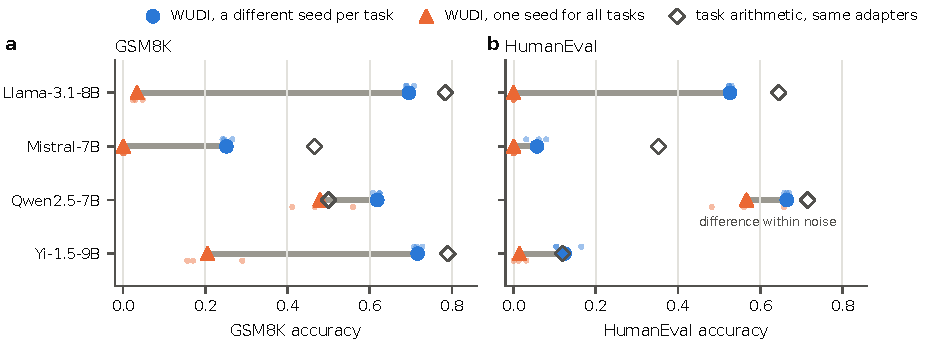
\includegraphics[width=\textwidth]{nc/figures/fig_wudi.pdf}
\caption{WUDI-Merging run as its authors run it, on each base model.
Triangles are cohorts created from one seed and circles cohorts with a seed
per task: large markers give the mean over three cohorts, small dots the
single cohorts. Open diamonds give task arithmetic on the same adapters,
averaged over both kinds of cohort, for reference. On Qwen2.5-7B at HumanEval
the difference is within the noise threshold (\S\ref{subsec:setup}); every
other difference clears it.}
\label{fig:wudi}
\end{figure}

The published procedure fails (Figure~\ref{fig:wudi}; Table~\ref{tab:wudi}
gives all three versions). Its worst-task excess is
$14.9$, $47.6$, $6.3$ and $4.7$ times larger on shared cohorts than on
independent ones, on Llama, Mistral, Qwen and Yi. Each ratio clears the noise
threshold, so the prediction that the optimiser protects WUDI fails on all four bases.
Accuracy follows. On GSM8K the shared cohorts score lower on every base,
down to $0.034$ against $0.695$ on Llama-3.1-8B. On HumanEval shared cohorts are worse, beyond the noise threshold, on
three of four bases, and on Llama and Mistral they score zero in every shared
cohort. The
closed form is exposed, as predicted: it is $5.3$ to $65$ times worse in NLL,
and worse on GSM8K on every base. On independent cohorts all three versions
leave a worst-task excess of only $0.03$ to $0.16$ nats. Run as published on
a collapsed cohort, WUDI returns a broken model and gives no warning.

The mechanism we had predicted for this failure did not hold. The closed form
does not concentrate its energy in the ill-conditioned directions, and the
3000-step version does not lie between the other two on two of the four bases.
Two diagnostics, recorded but not pre-registered, separate the two kinds
of cohort instead. On shared cohorts Adam drives the merged update from $4$ to between
$8.6$ and $12.5$ times the norm of the mean update. There, $24$ to $27\%$ of
its squared norm lies outside the row space of the $A_t$, where the loss
cannot see it, against $0.8$ to $1.6\%$ on independent cohorts
(Appendix~\ref{app:wudi-diag}).

\subsection{Where each merge puts its energy}\label{subsec:energy}

\begin{figure}[pos=tbp]
\centering
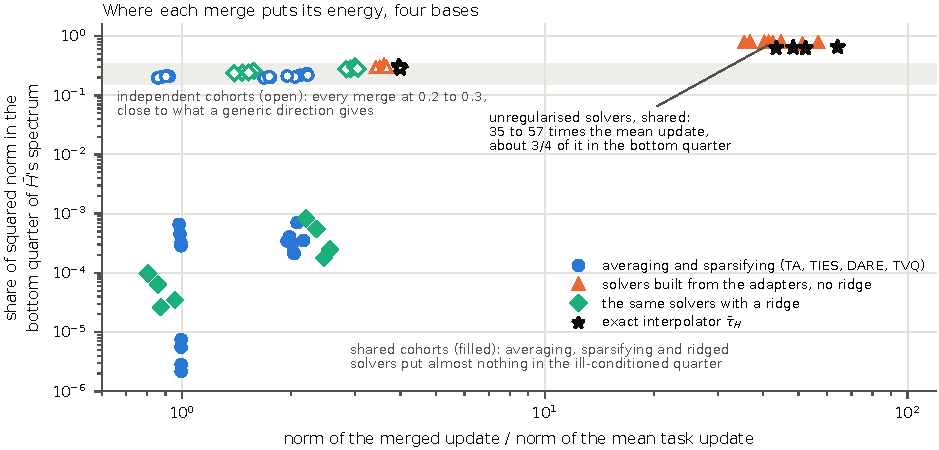
\includegraphics[width=\textwidth]{nc/figures/fig4_mechanism.pdf}
\caption{Where each merged solution puts its energy, on the four bases. Each
point is one method on one base; filled markers are the shared cohort, open
markers the independent one. Horizontal: norm of the merged update relative to
the mean task update. Vertical: share of its squared norm in the bottom quarter
of $\bar H$'s spectrum, the ill-conditioned directions. ``The same solvers with
a ridge'' are adapter-only RegMean at $\lambda = 0.13$ and our encoder at
$\lambda = 0.05$.}
\label{fig:mechanism}
\end{figure}

For the other methods the mechanism can be checked without any forward pass,
because every merge is arithmetic on the adapter factors
(Figure~\ref{fig:mechanism}). On shared cohorts, every averaging and
sparsifying merge is at most $2.2$ times the norm of the mean task update.
It puts almost none of its energy (less than $0.001$) in the bottom quarter
of $\bar H$'s spectrum. The two unregularised solvers built from the adapter
factors are $35$ to $57$ times the mean update and put $73$ to $80\%$ of
their energy there. Among these methods, they are the only ones that
enter the ill-conditioned directions, and a ridge brings them back down beside
the heuristics. On independent cohorts every method puts $0.20$ to $0.32$ of
its energy in the bottom quarter, close to what a direction unrelated to the
spectrum gives. WUDI is the exception to this picture (\S\ref{subsec:wudi}): it
is amplified on shared cohorts without concentrating in those directions.

\subsection{The other methods}\label{subsec:results}

\begin{table}[pos=tbp]
\centering
\small
\caption{Which merges the collapse reaches. Each method is compared with itself
on shared and independent cohorts, three of each kind on four bases. NLL is the
ratio of worst-task excess, shared over independent, over the four bases.
Accuracy is GSM8K exact match and HumanEval pass@1; for MaTS it uses one cohort
of each kind. KnOTS is its TIES variant, and diagonal Fisher uses the squared update
as a data-free proxy for the Fisher. The prediction was registered before any
of the methods we did not build was run.}
\label{tab:exposure}
\setlength{\tabcolsep}{3.5pt}
\begin{tabularx}{\textwidth}{>{\raggedright\arraybackslash}p{2.5cm}
                >{\raggedright\arraybackslash}p{1.7cm}
                >{\raggedright\arraybackslash}p{1.5cm}
                >{\raggedright\arraybackslash}X
                >{\raggedright\arraybackslash}X}
\toprule
method & matrix built from & predicted & NLL, shared / indep. & accuracy \\
\midrule
task arithmetic, TIES, DARE, TVQ, KnOTS & no matrix & immune
  & no effect in 15 of 20 base--method pairs; largest $0.015$ nats
  & equivalent within $3$ points (GSM8K) and $5$ (HumanEval) \\
\addlinespace
RegMean, activation Grams & data & immune & $0.99$ to $1.14$
  & equal on all 8 base--benchmark pairs \\
MaTS & data (Fisher) & immune & $0.93$ to $0.99$
  & equal in 7 of 8; 1 favours shared \\
diagonal Fisher & task updates, diagonal & immune & $0.96$ to $1.08$ & not run \\
\addlinespace
TSV-M (whitening) & task updates & exposed & $0.81$ to $1.19$, mixed sign
  & no difference beyond the noise threshold \\
\addlinespace
WUDI, as published & task updates & protected by its optimiser & $4.7$ to $47.6$
  & GSM8K $0.00$ to $0.48$ vs.\ $0.25$ to $0.72$ \\
WUDI, closed form & task updates & exposed & $5.3$ to $65.1$
  & GSM8K $0.00$ to $0.18$ vs.\ $0.27$ to $0.72$ \\
\addlinespace
RegMean, adapter-only & adapter factors & exposed & $1.8$ to $65.6$
  & GSM8K $0.00$ to $0.17$ vs.\ $0.29$ to $0.72$ \\
our encoder & adapter factors & exposed & $2.5$ to $66$
  & Mistral $0.000$ on both \\
\bottomrule
\end{tabularx}
\end{table}

\begin{figure}[pos=tbp]
\centering
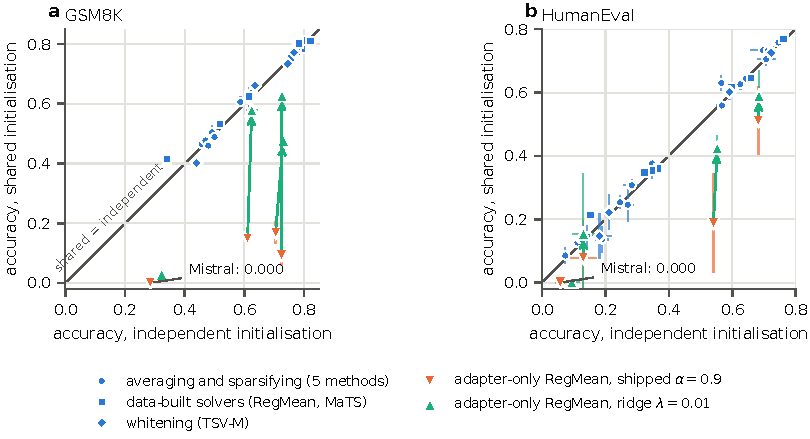
\includegraphics[width=\textwidth]{nc/figures/fig5_accuracy.pdf}
\caption{Downstream accuracy on shared against independent cohorts. Each point
is one method on one base model, the mean over three cohorts of each kind, with bars
of one standard deviation across cohorts. Points on the diagonal are unaffected
by the initialisation. Every published method shown lies on or near it;
adapter-only RegMean at its shipped setting ($\alpha = 0.9$) lies far below it.
Arrows go from that setting to the same solver with a ridge of
$\lambda = 0.01$ on the same base, which recovers most of the GSM8K loss on
three bases and not on Mistral. WUDI is in Figure~\ref{fig:wudi}.}
\label{fig:exposure}
\end{figure}

Table~\ref{tab:exposure} and Figure~\ref{fig:exposure} give the outcome for
every method.

\paragraph{Averaging and sparsifying merges are unaffected.} In NLL, $15$ of
the $20$ pairs of base model and method show no difference beyond the noise
threshold, which here sits near $0.01$ nats. The five differences that clear
it are small and favour independent cohorts. Three of them are KnOTS, which aligns subspaces and so acts
most directly on subspace geometry of all the heuristics. Finding no difference at
hundredths of a nat is weak evidence, so for accuracy we registered an
equivalence test (two one-sided tests, three cohorts of each kind, $240$
evaluations). All five heuristics are equivalent across regimes within
margins, fixed in advance, of $3$ points on GSM8K and $5$ on HumanEval. The equivalence is
a statement about means over the four bases. Taken alone, one of the $40$
combinations of method, base and benchmark exceeds its margin: TIES on Llama
at HumanEval, where shared cohorts score $6.5$ points higher.

We had also predicted that a slight lean towards shared cohorts, seen with
one cohort of each kind, would vanish with three. It persisted, at a mean of $0.7$
points with all four bases leaning the same way (a permutation test over
cohorts gives $p = 0.007$). Rank truncation, the explanation we tested in
advance, does not account for it, and we have no tested explanation
(Appendix~\ref{app:lean}). In practice, a heuristic merge loses
nothing to a shared initialisation.

\paragraph{Solvers built from data, and a diagonal one, are unaffected.} We
ran three such methods on all six cohorts of each base. They are RegMean with
real activation Grams at its published setting, MaTS with its
blockwise Fisher solved by conjugate gradient, and diagonal Fisher merging.
Our diagonal Fisher weights each coordinate by its squared update, a
data-free proxy, so its matrix comes from the task updates. Being diagonal, it
cannot see overlap between subspaces. The three immunity predictions hold.
RegMean shows no effect on any base in either unit. Averaged over the two
benchmarks, it is the most accurate merge in our experiments on three of the
four bases. Its accuracy on the two kinds of cohort agrees within $1.3$
points for every base and benchmark. MaTS shows no NLL effect, and in accuracy one
comparison (Mistral, GSM8K) favours shared cohorts. Diagonal Fisher shows one small
effect, $1.08$ times on Llama. With the activation data it was
designed for, RegMean is safe on a collapsed cohort.

\paragraph{Whitening is not affected, against our prediction.} We predicted
that TSV-M would be exposed. It shows an NLL effect on Mistral only ($1.19$
times), one in the opposite direction on Yi, and none on Llama and Qwen. No
accuracy difference clears the noise threshold. The prediction failed. Whitening
orthogonalises the stacked singular vectors rather than solving a
least-squares problem in them, and the rule in \S\ref{subsec:rule} is stated
for least-squares merges alone.

\paragraph{Solvers built from the adapter factors fail.} The data-free form of
RegMean replaces each activation Gram by $A_t^\top A_t$. It is a variant we
constructed, not the published method. It is the natural choice when only the
adapter files are available. With a minimal ridge ($\lambda = 10^{-6}$) its
worst-task excess (Figure~\ref{fig:ridge}, top row) is $4.1$, $65.6$, $5.8$
and $1.8$ times larger on shared cohorts on Llama, Mistral, Qwen and Yi. The
gain from tuning the ridge is larger on shared cohorts on all four. Both
results match our predictions. In accuracy, with RegMean's own
shipped regulariser ($\alpha = 0.9$) and no added ridge, shared cohorts score
at most $0.17$ on GSM8K, against $0.29$ to $0.72$ for independent ones. On Mistral it scores zero on both
benchmarks in all three shared cohorts. On shared cohorts, a ridge of
$\lambda = 0.01$ beats the shipped setting beyond the noise threshold on
GSM8K on three of four bases, by $31$ to $54$ points on Llama, Qwen and Yi.
On HumanEval it does so on two bases. It does not rescue Mistral ($0.029$ and $0.002$),
whose NLL sweep selects $\lambda = 0.05$. A value of $0.01$ is therefore a
starting point for a sweep, not a recommended value.

The second solver of this kind is the closed-form encoder of our earlier
preprint~\citep{pathak2026rd}, which we call \emph{our encoder}. It computes
the exact interpolator $\tauH = \bar D\,\bar H^{+}$ of \S\ref{sec:background}
directly, with an optional ridge on the range of $\bar H$, so it inverts the
collapsed operator itself. Without a ridge it is $2.5$ to $66$ times worse on
shared cohorts, beyond the noise threshold on every base. On Mistral
its merged model scores $0.000$ on both benchmarks, and a tuned ridge brings
this up to $0.46$ on GSM8K and $0.23$ on HumanEval. The effect survives with
rank truncation disabled, where the ratio grows to $25$ to $117$. Truncating
to rank $r$ discards most of the ill-conditioned subspace and so hides part of
the damage. For both solvers, the amount of ridge needed does not track the
conditioning, while the amount it buys does. The selected $\lambda$ is the
same on the two kinds of cohort on three of four bases for the encoder, and on two for
adapter-only RegMean.

\paragraph{Numerical precision.} Both solvers run in float32, and at
$\lambda = 10^{-6}$ and $\lambda = 0$ their systems are badly conditioned,
so the failure could in principle be rounding error. It is not. A registered
check recomputed both solvers' merges at these settings in float64, on every
base and for both kinds of cohort. The ratio of shared to independent
amplification agreed with float32 within $0.1\%$ in every case. One merge
fell outside the tolerance set in advance, the encoder on the shared Yi
cohort. Rebuilt in float64, it fails as before: $0.245$ nats, against $0.249$
in float32 and $0.121$ on the independent cohort. The unregularised float32
encoder is, however, sensitive to the random seed of its randomised SVD. Over
repeated draws, the shared cohorts always stay worse than the independent
one. On Yi, though, the ratio between them ranges from $1.8$ to $2.6$ over the
draws. The predicted factor of two therefore holds on the registered runs but
not on every draw (Appendix~\ref{app:precision}).

\subsection{Why RegMean's shipped regulariser does not fix it}\label{subsec:default}

RegMean scales the off-diagonal entries of each Gram by $\alpha$, by default
$0.9$. Up to an overall factor of $\alpha$ that cancels in the solve, this is
equivalent to adding $\frac{1-\alpha}{\alpha}\operatorname{diag}(G)$. That is
a shrinkage whose size is set by the scale of the data, not by the
conditioning. It was designed for activation Grams, and here we apply it
outside that use. On the adapter Grams it has the average size of an
isotropic ridge of $5.8\times10^{-4}$ to $6.8\times10^{-4}$, the same on both
kinds of cohort to within $0.5\%$ (Figure~\ref{fig:ridge}, bottom row). On
independent cohorts that amount leaves a condition number of $1.2\times10^{3}$ to
$1.4\times10^{3}$. On shared cohorts it leaves $6.6\times10^{3}$ to
$9.1\times10^{3}$, while $\lambda = 0.01$ brings the same layers to about
$1.5\times10^{2}$. The shipped setting applies the same amount whatever the
regime. That amount is ample on a separated cohort and an order of magnitude too small
on a collapsed one, and nothing in the method signals the difference. A user
can lower $\alpha$; the default does not.

\begin{figure}[pos=tbp]
\centering
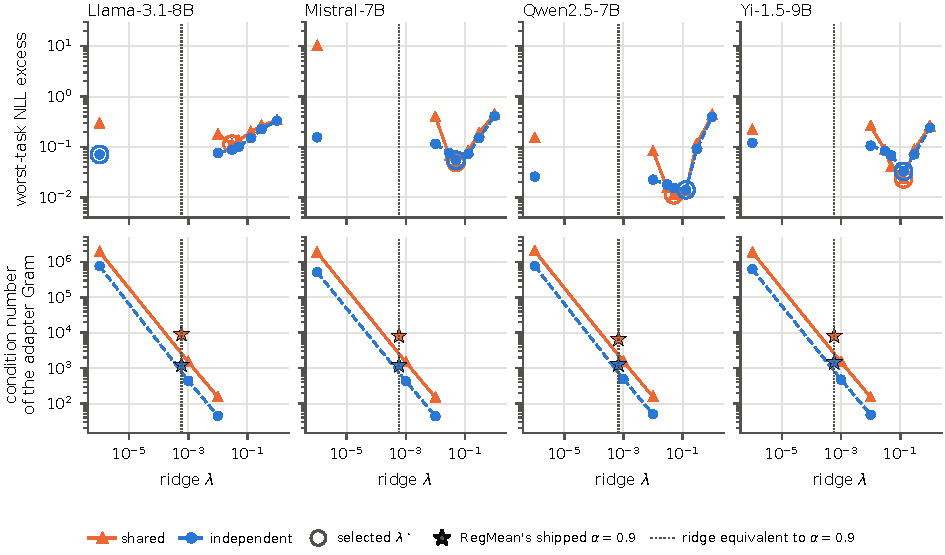
\includegraphics[width=\textwidth]{nc/figures/fig6_ridge.pdf}
\caption{Adapter-only RegMean against an added isotropic ridge $\lambda$, per
base model, on one shared and one independent cohort. \textbf{Top:} worst-task
NLL excess; circles mark the selected $\lambda^\star$, and the point at
$\lambda = 10^{-6}$ is not joined to the rest because no grid point lies
between. \textbf{Bottom:} condition number of the adapter Gram. Stars mark
RegMean's shipped $\alpha = 0.9$, placed at the isotropic ridge of the same
average size, $(1-\alpha)/\alpha$ times the mean diagonal of the Gram (dotted). That
size is the same for both kinds of cohort, and on the shared cohort it
leaves a higher
condition number than an isotropic ridge of that size would.}
\label{fig:ridge}
\end{figure}

\subsection{A vision model, and all four tasks}\label{subsec:beyond}

\paragraph{A vision model.} We repeated the central comparisons on CLIP
ViT-B/32 with eight image classification tasks (SUN397, Cars, RESISC45,
EuroSAT, SVHN, GTSRB, MNIST and DTD). We trained rank-$16$ adapters in three
shared and three independent cohorts, merged them as dense updates without
truncation, and scored mean top-1 accuracy over the eight tasks. Every
prediction made in advance holds. The shared cohorts sit at median cosine $0.96$
and the independent ones at $0.11$. Adapter-only RegMean fails
as on language models, scoring $0.043$ on shared cohorts against $0.369$ on
independent ones, and a ridge of $\lambda = 0.1$ repairs it ($0.735$ against
$0.747$). Task arithmetic and TIES are equivalent within two points, and
activation-Gram RegMean and TSV-M show no effect beyond the noise threshold
(Table~\ref{tab:appC-vision}). WUDI's closed form fails, $0.045$ against
$0.369$. Published WUDI does not fail here.
Shared cohorts merge \emph{better} with it, $0.454$ against $0.358$. The
difference is well beyond the noise threshold and in the opposite direction to
the language models. We had predicted only an absence of harm, which this
outcome satisfies. We did not predict a reversal, however, and we cannot explain
it. It remains an open question about the exposed class.

\paragraph{All four tasks.} The accuracy results so far cover mathematics
and code. We also tested the other two tasks, with our encoder on one
cohort of each kind. On translation (WMT19, chrF) the collapse is visible. On
the shared cohort the selected ridge beats $\lambda = 0$ by $2.9$ to $55.1$
chrF points, beyond the noise threshold on all four bases. Task arithmetic and
TIES differ between the two kinds by at most $1.1$ points. On IFEval it is not visible. The
instruction adapter alone does not beat the base model there on three of
four bases, so there is little task skill for a broken merge to lose
(Appendix~\ref{app:alltasks}).

\subsection{Two open problems}\label{subsec:open}

\paragraph{Setting the ridge without data.} A ridge repairs both solvers
built from the adapter factors on most bases, but the amount needed does not
track the conditioning. We tested three data-free rules for choosing it:
one that targets a condition number, generalised cross-validation and the
L-curve. All three failed the criteria we set in advance
(Appendix~\ref{subsec:lambda}). We recommend starting at $\lambda = 0.01$
and sweeping on held-out data.

\paragraph{Public cohorts.} We also merged public cohorts selected by a
fixed rule. Unregularised adapter-only RegMean at least doubles task
arithmetic's excess on $5$ of $6$ collapsed cohorts, and also on $11$ of $13$
separated ones (Fisher's exact test, $p = 0.78$). The solver fails often on
public adapters, but not more often when they are collapsed, so these merges
show how common the collapse is (\S\ref{sec:prevalence}), not what it costs
there. We tested two candidate causes on our own cohorts. The freedom in
LoRA's factorisation does not matter. A fourfold scale mismatch between
adapters does harm the solver, which we did not predict, but it does not
explain the public failures, which remain unexplained
(Appendix~\ref{subsec:against}).

\subsection{The rule}\label{subsec:rule}

We tested twelve methods, ten of them published methods we did not build.
The collapse reaches exactly the merges that solve a least-squares problem whose
matrix is built from the adapters alone, in closed form or by gradient
descent. That matrix can come from the adapters' factors or from the task
updates they define. The class includes a published method run exactly as its
authors run it. The collapse does not reach averaging or sparsifying merges,
solvers whose matrix is built from data, a diagonal solver, or whitening.
